\section{Results and Observations}

\subsection{Determination of Truss Inertia}

The truss inertia as estimated by SolidWorks is $0.00192 \,\,kg\,m^2$.
The truss inertia determined through various experiments is listed in Table \ref{tbl:inertia}.

\begin{table}[htb]
	\centering
	\caption{Truss Inertia Experimental Results}
	\label{tbl:inertia}
	\vspace{6pt}
	\footnotesize
	\begin{tabular}{cccc}
		\toprule
		Applied Voltage & Magnet As Load & Inertia & Average \\
		\midrule
		5 V & No & 0.00398  \\
		7.5 V & No & 0.00361& 0.00347 \\
		9 V & No & 0.00349 \\
		\midrule
		5 V & Yes & 0.00392 \\
		7.5 V & Yes & 0.00329 & 0.00369\\
		9 V & Yes & 0.00319 \\
		\bottomrule
	\end{tabular}
\end{table}

The difference between theoretical  (0.00192) and experimental (0.00347) values is roughly a factor of 2. 
There are at least two explanations for the difference. 
Firstly, the truss rods were soldered at the joints, which adds extra weight that the computer model does not account for. 
Secondly, the actual truss inertia is an experimental value using all the data sheet parameters provided by the motor manufacturer. These parameters cannot be assumed to be accurate for every individual motor. 

\subsection{Controller Design}

System response to position control may be seen in Figure \ref{fig:positionresponse} on page \pageref{fig:positionresponse}.
Although settling time and overshoot are set to be $T_s = 0.6$ and $PO = 0.15$, the response is observed to have larger the settling time and maximum overshoot values.
There are many possible causes for this discrepancy.  
First, the new zero in the transfer function, created by adding derivative gain, was ignored. 
The reason that we made this assumption to ignore the zero is to equate the ideal transfer function with our PD transfer function to determine $\zeta$ and $\omega_n$. 
Secondly, it is known that $\zeta$ has significant effect percent overshoot and also $\zeta$ and $\omega_n$ affect the settling time.
For these reasons overshoot and settling time of the system response are different for their original values.

\begin{figure}[ht]
    \centering
    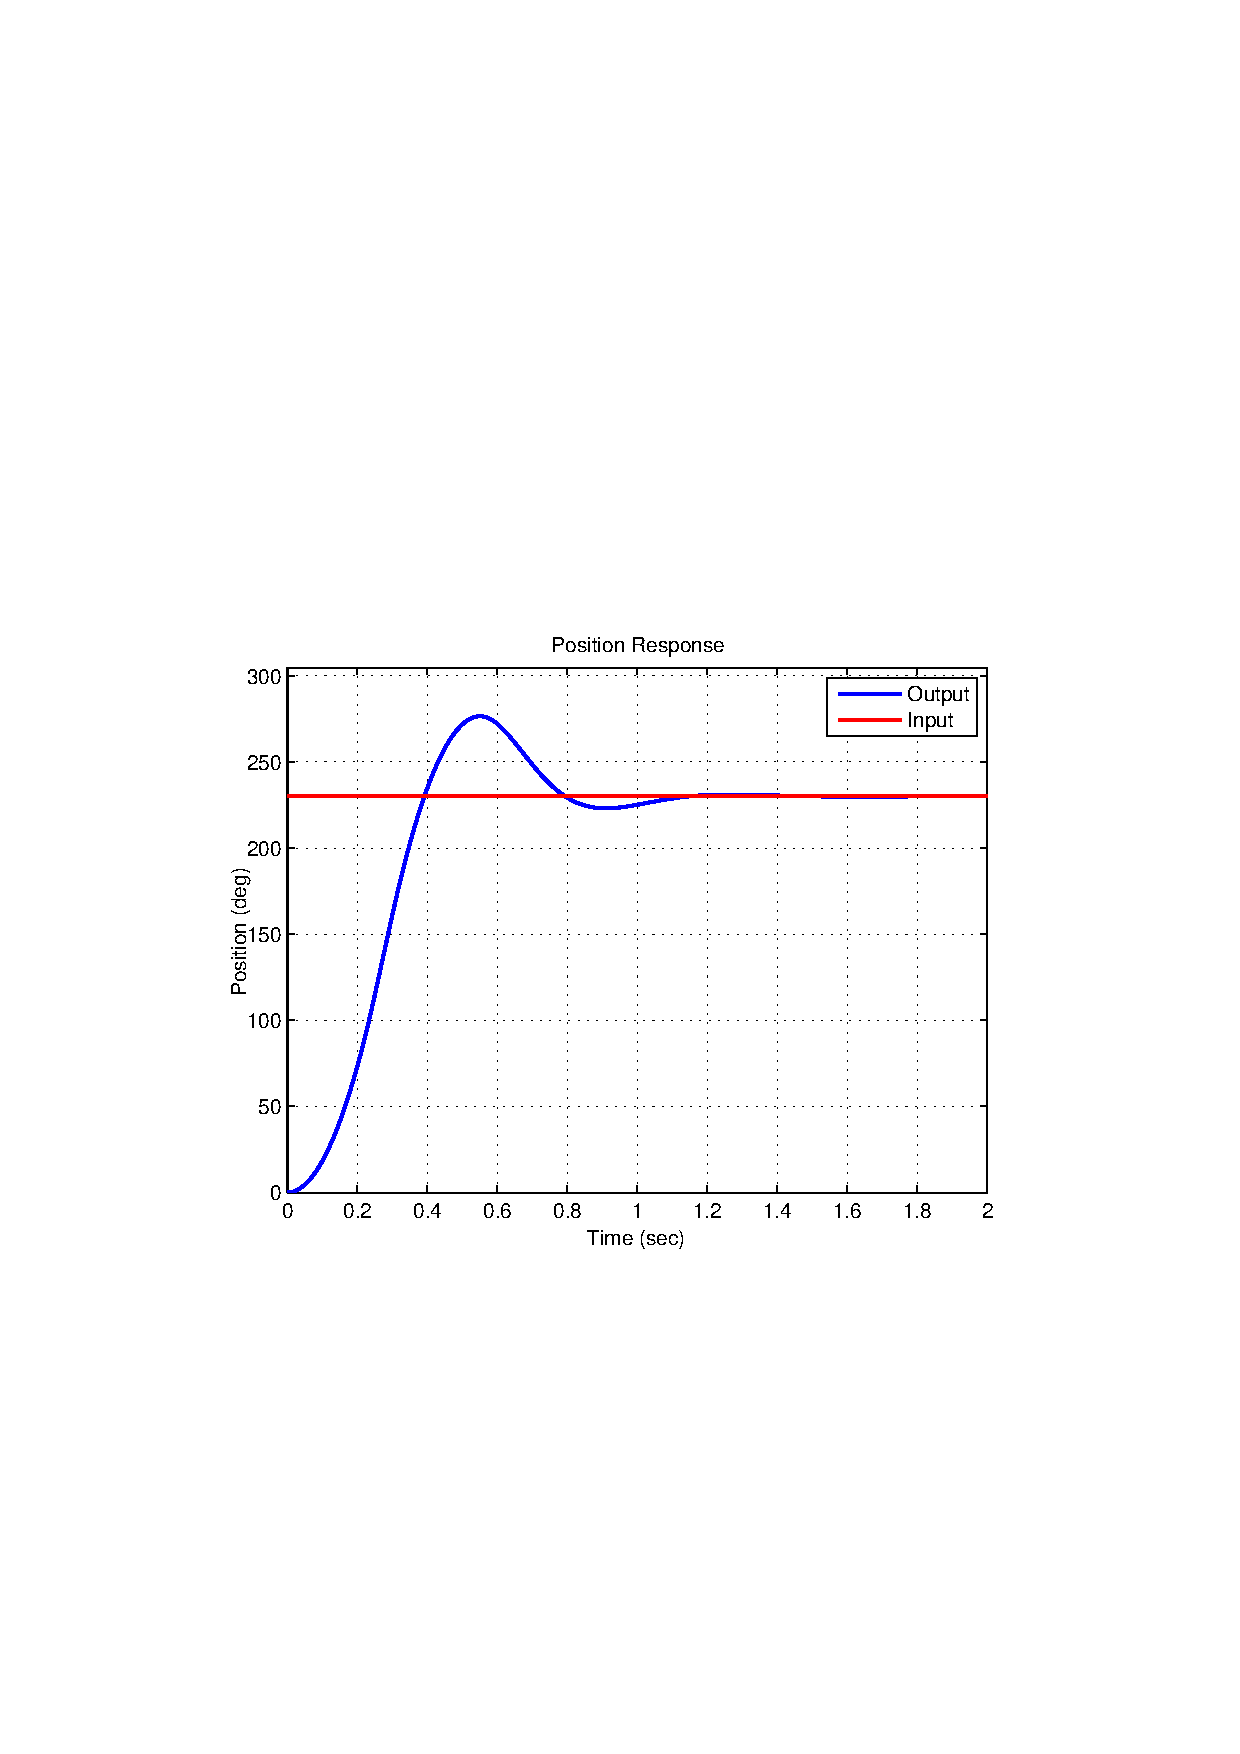
\includegraphics[width=.99\textwidth]{images/response.pdf}
    \caption{Position Response}
    \label{fig:positionresponse}
\end{figure}

\subsection{Amplifier Compensation}

Figure \ref{fig:amp} shows amplifier output voltage for a given input voltage over time.
Data was captured with the motor connected to the amplifier.
Throughout the experiment variable load was applied to the motor; it can be seen that load had little effect on output voltage and therefore speed.

\begin{figure}[ht]
    \centering
    \includegraphics[width=.99\textwidth]{images/amplifier.pdf}
    \caption{Amplifier Input and Measured Voltage vs Time}
    \label{fig:amp}
\end{figure}
